\section{CFD analýza konstrukčních úprav} \label{sec:konstrukcni-upravy}
    TODO
    
    \subsection{Studie citlivosti výpočetní sítě}
        TODO
    \subsection{Sonda bez stínění čidla B}
        Analýzu konstrukčních úprav zahájilo zkoumání nejjednodušší varianty sondy – s původními rozměry stínění čidla A a bez jakéhokoli odstínění čidla B. Cílem bylo určit problematická místa, která bude vhodné zkoumat jako první. Použitý model je znázorněn na obrázku \ref{fig:sonda-bez-stineni-B}, konkrétní rozměry jsou uvedeny v příloze \ref{fig:sonda-bez-stineni-B-vykres}. Zkoumáno bylo chování restitučních faktorů při různých rychlostech nabíhajícího proudu v rozmezí $100 \div 325 \unit{\frac{m}{s}}$ a při vychýlení sondy ve dvou rovinách – v rovině symetrie $XY$ (natočení značeno jako $\varphi _Z$) a poté kolmo na rovinu symetrie (rovina $XZ$, značeno $\varphi _Y$).
        
        \begin{figure}[ht!]
            \centering
            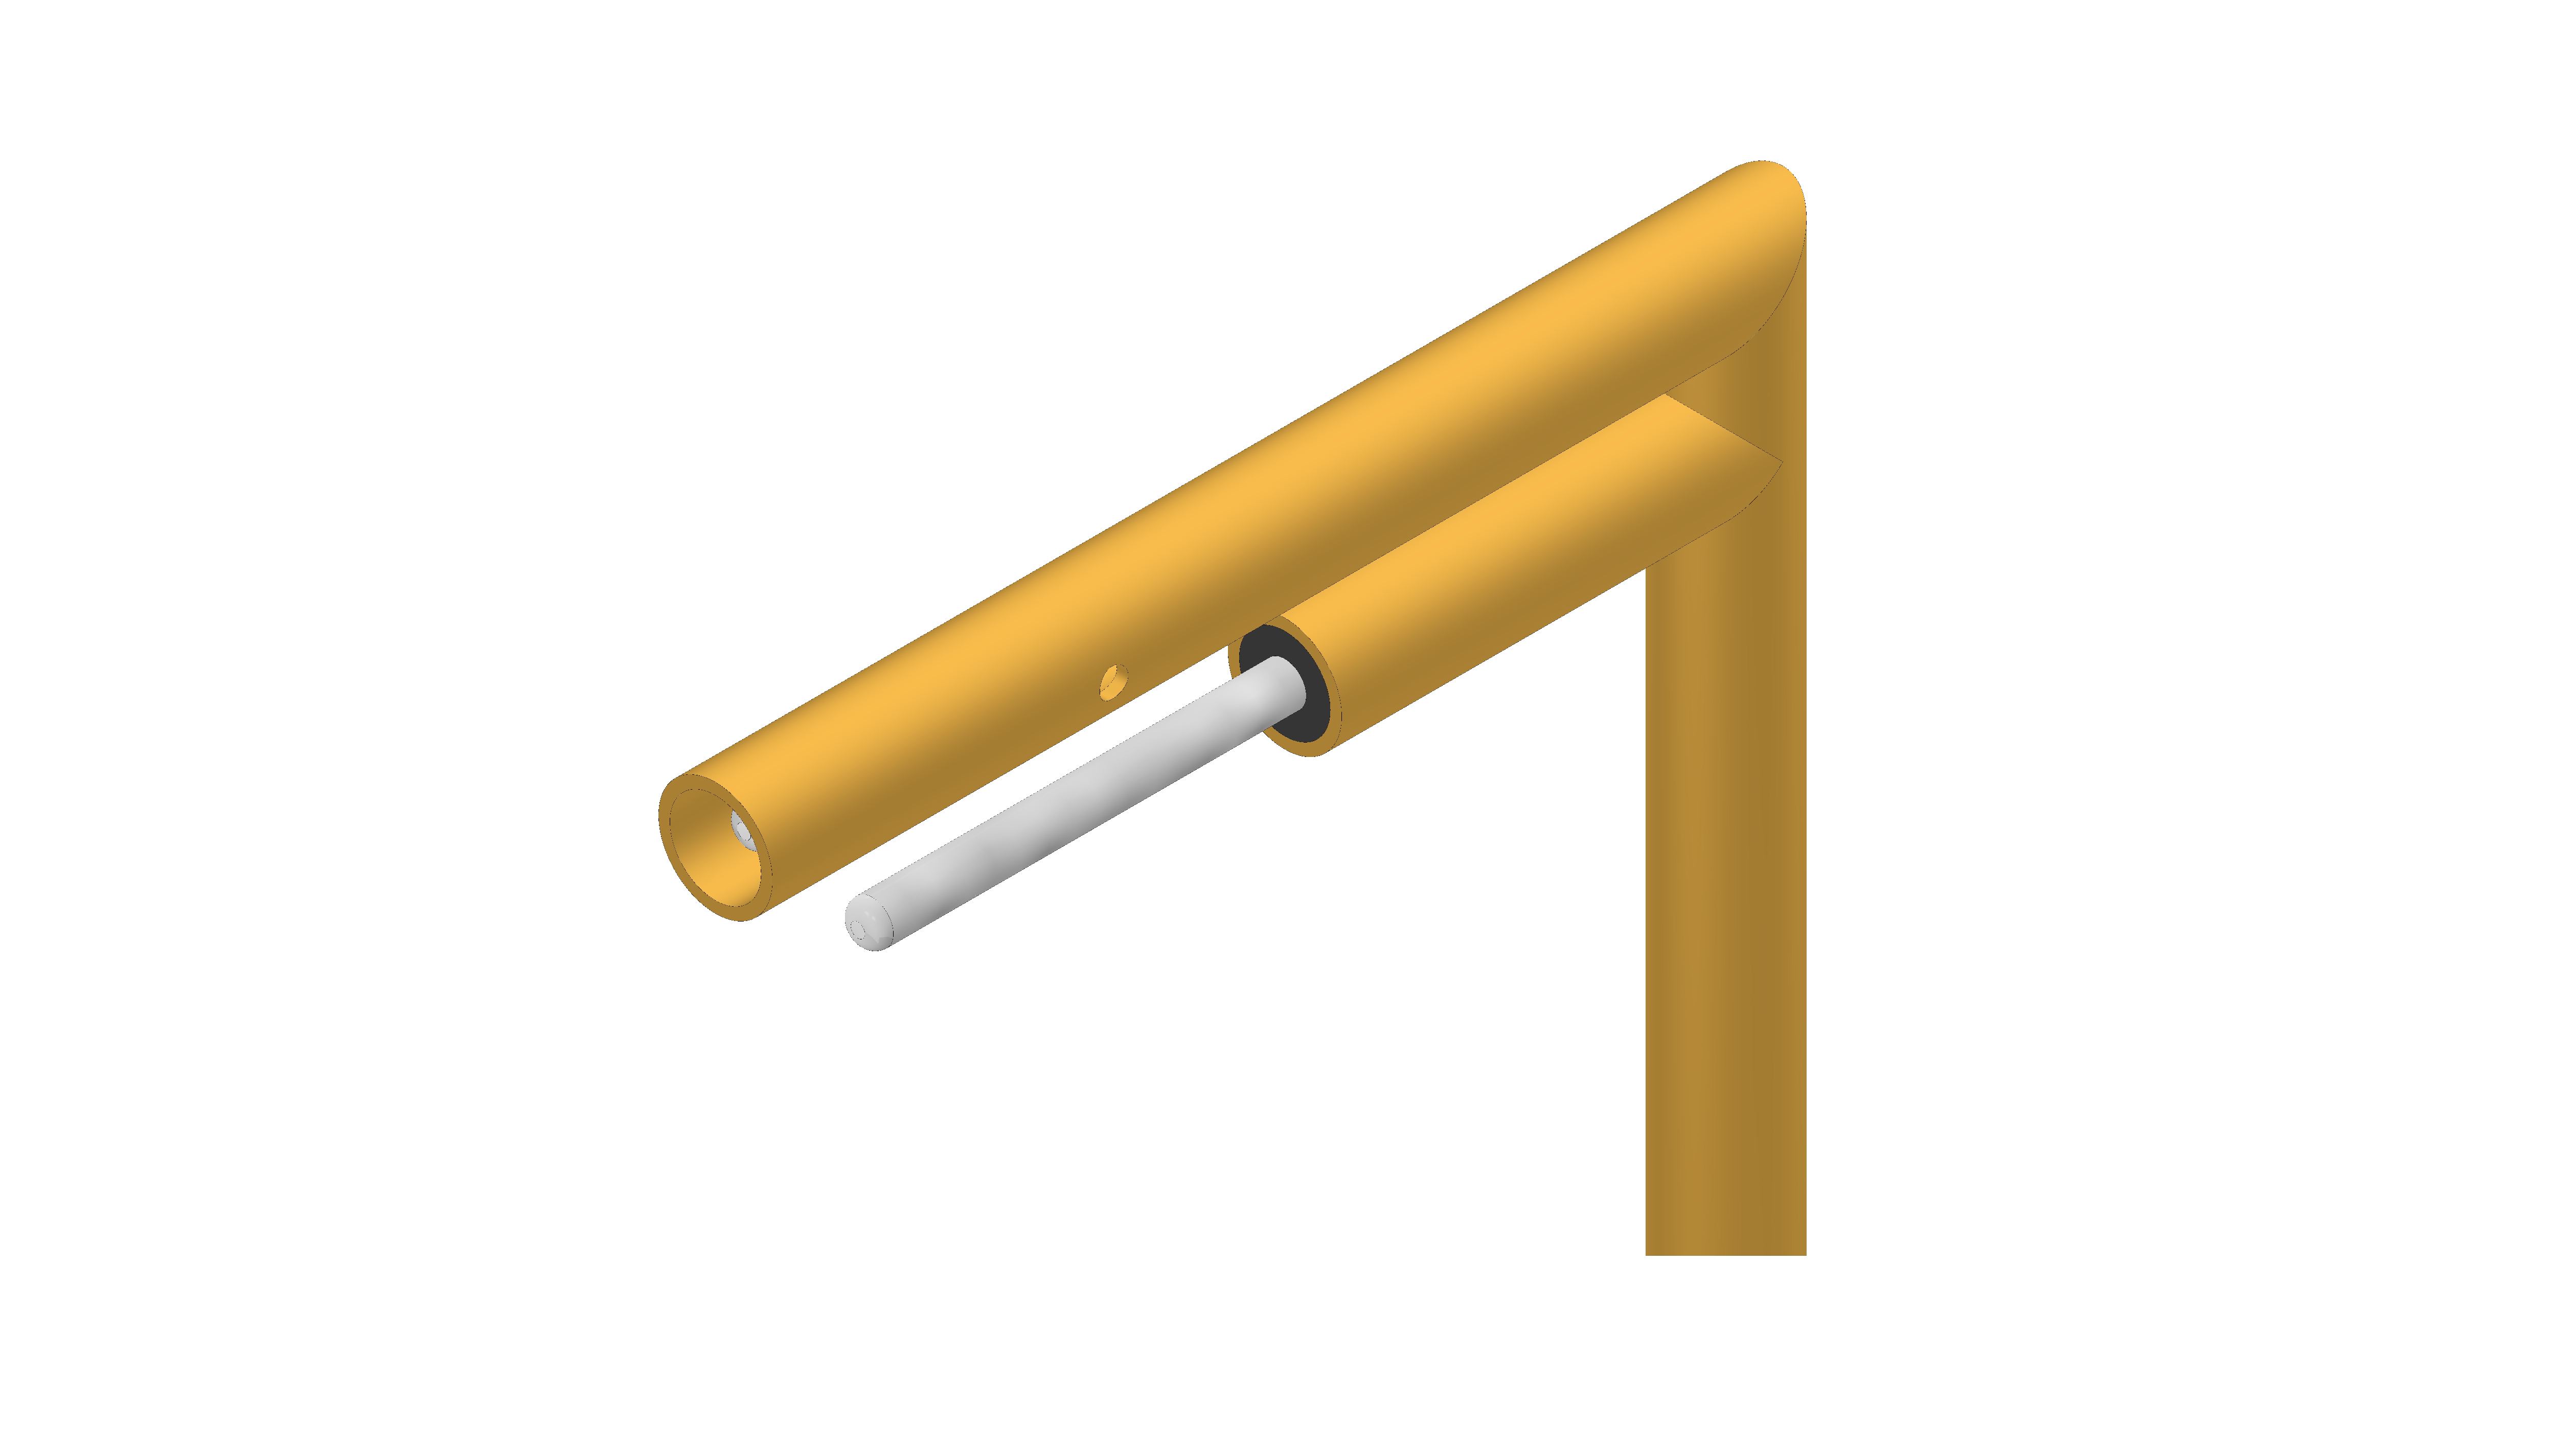
\includegraphics[width=\textwidth]{400_SIMULACE_KONSTRUKCNICH_UPRAV/Vykresy_rendery/Sonda_bez_stineni_B.png}
            \caption{Sonda bez stínění čidla B}
            \label{fig:sonda-bez-stineni-B}
        \end{figure}
        \subsubsection{Chování při různých rychlostech proudění}
            Výpočet byl proveden s následujícími okrajovými podmínkami:
            
            \begin{figure}[ht!]
                \centering
                \includegraphics*[width=\textwidth, trim={5.9cm 1.0cm 5.7cm 2.0cm}]{400_SIMULACE_KONSTRUKCNICH_UPRAV/Grafy/01_rychlosti.eps}
                \caption{Závislost restitučních faktorů sondy bez stínění čidla B na rychlosti proudění}
                \label{fig:sonda-bez-stineni-rychlosti}
            \end{figure}
        \subsubsection{Směrová citlivost v rovině symetrie}
            DATA
            
            \begin{figure}[ht!]
                \centering
                \includegraphics*[width=\textwidth, trim={5.9cm 1.0cm 5.8cm 2.0cm}]{400_SIMULACE_KONSTRUKCNICH_UPRAV/Grafy/01_rovina_symetrie}
                \caption{Závislost restitučních faktorů sondy bez stínění čidla B na natočení sondy v rovině symetrie}
                \label{fig:sonda-bez-stineni-rovina-symetrie}
            \end{figure}
        \subsubsection{Směrová citlivost kolmo na rovinu symetrie}
            DATA
            
             \begin{figure}[ht!]
                \centering
                \includegraphics*[width=\textwidth, trim={5.9cm 1.0cm 5.8cm 2.0cm}]{400_SIMULACE_KONSTRUKCNICH_UPRAV/Grafy/01_kolma_rovina}
                \caption{Závislost restitučních faktorů sondy bez stínění čidla B na natočení kolmo na rovinu symetrie}
                \label{fig:sonda-bez-stineni-kolma-rovina}
            \end{figure}
    \newpage
    \subsection{Sonda se stíněním čidla B}
        DATA
        
        \begin{figure}[ht!]
            \centering
            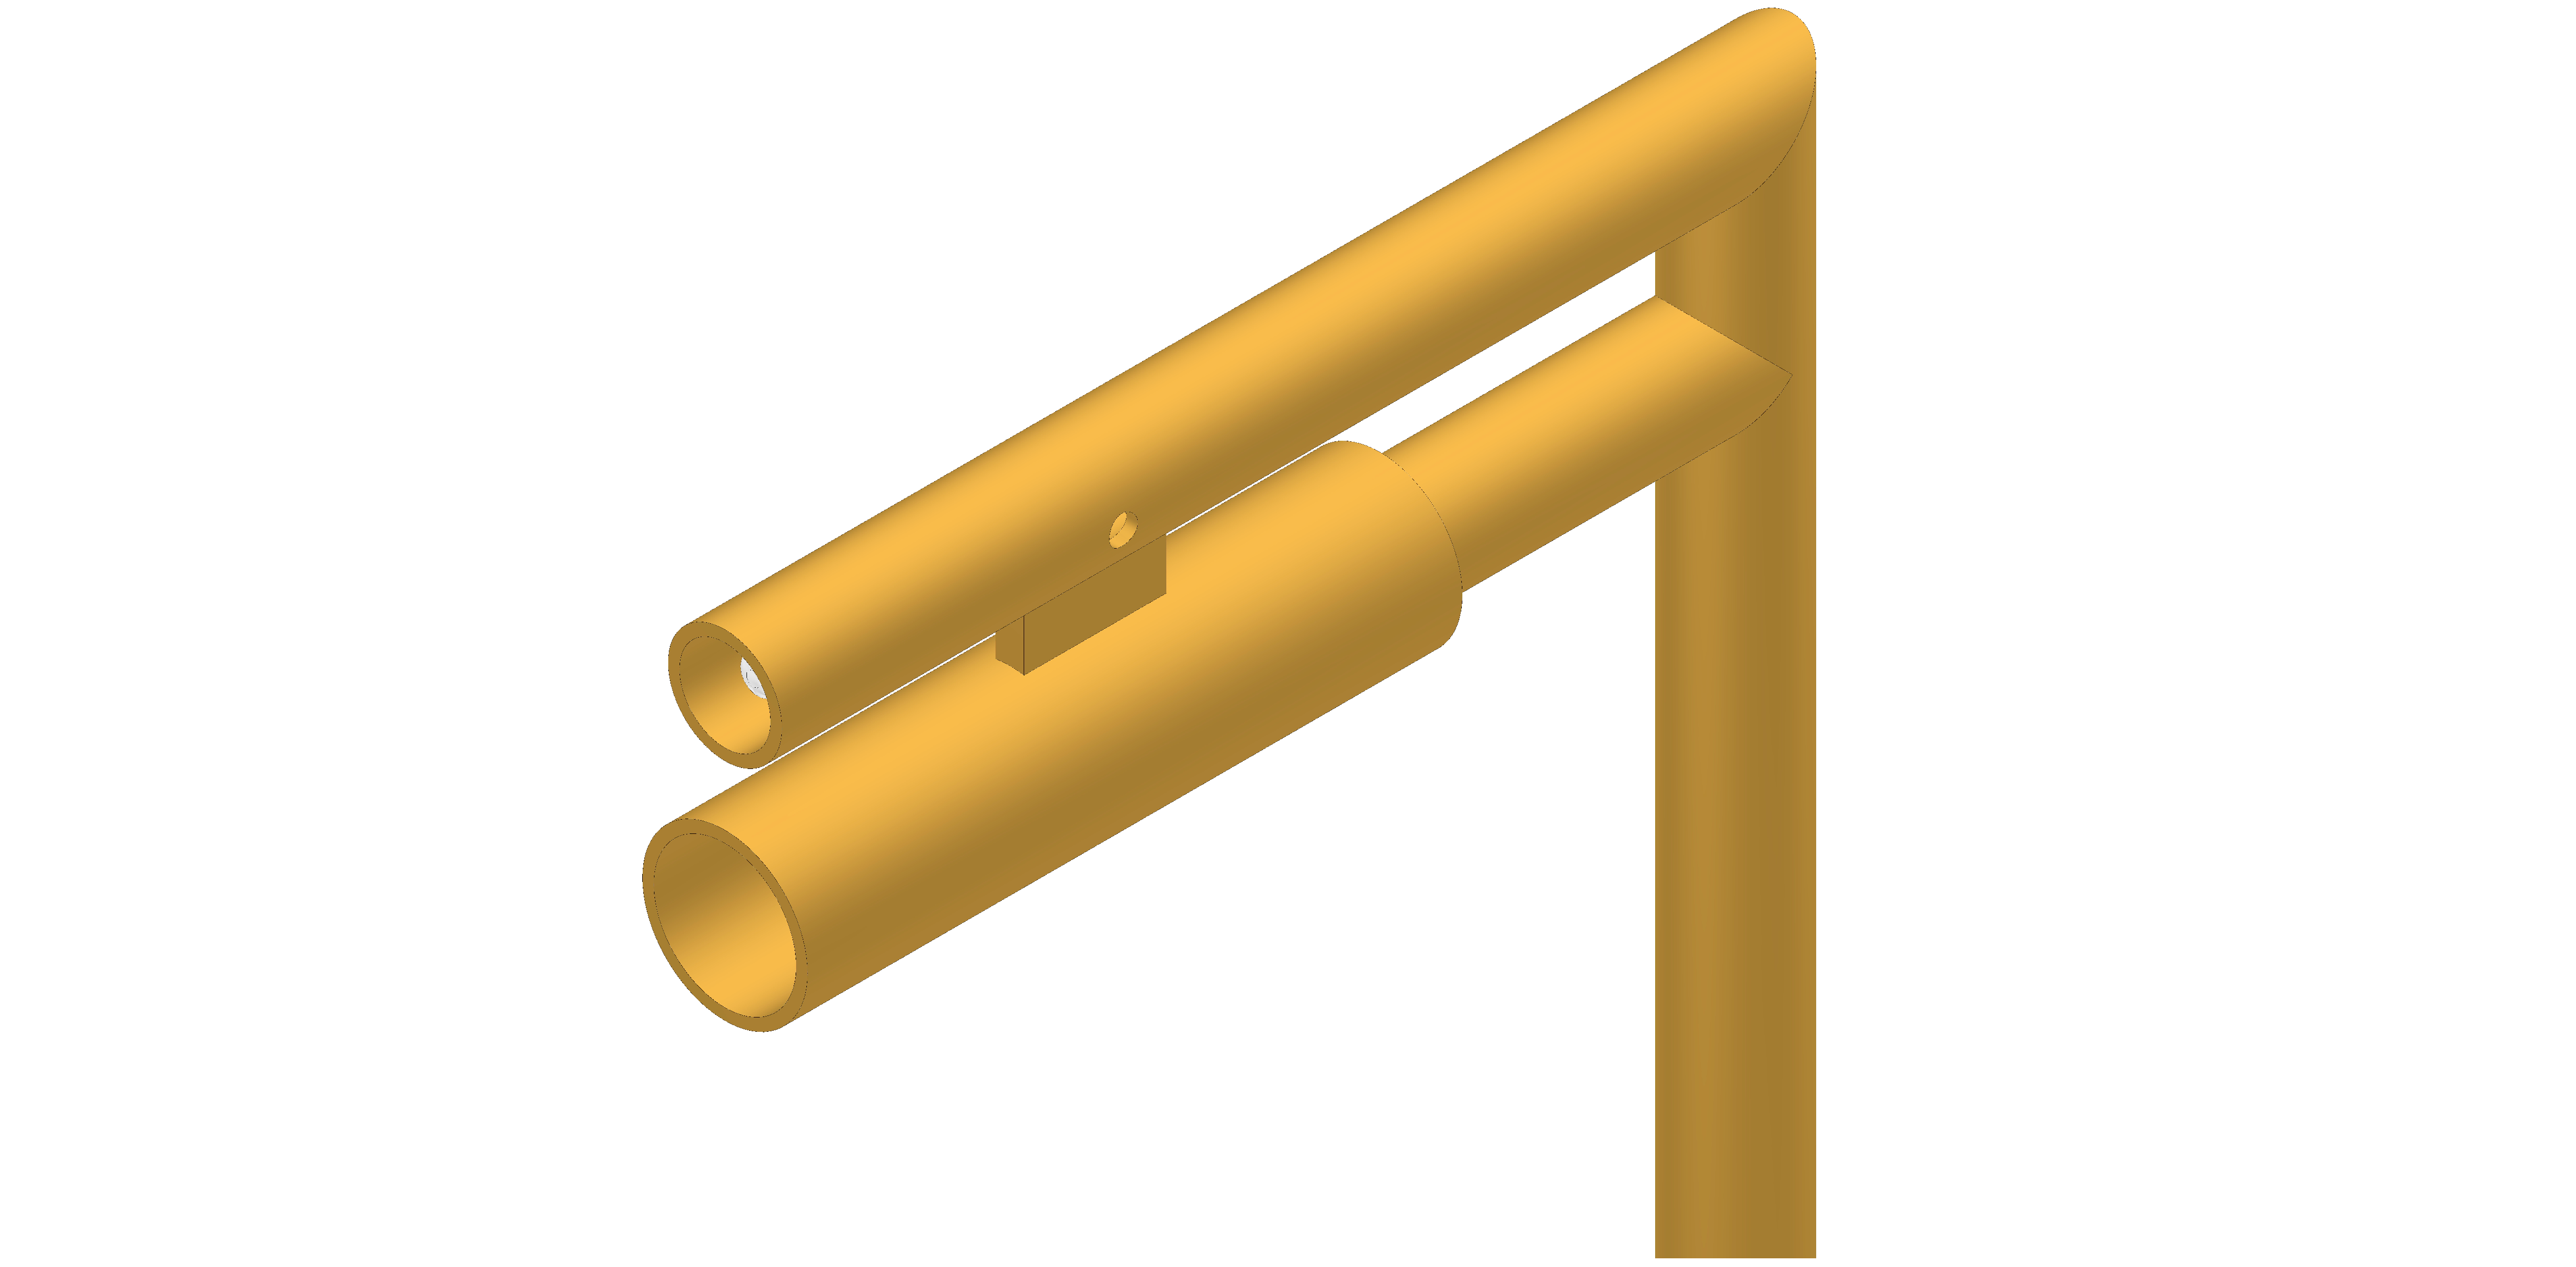
\includegraphics[width=\textwidth]{400_SIMULACE_KONSTRUKCNICH_UPRAV/Vykresy_rendery/Sonda_se_stinenim_B.png}
            \caption{Sonda se stíněním čidla B}
            \label{fig:sonda-se-stinenim-B}
        \end{figure}
    
    \newpage
    \subsection{Sonda s rozšířeným stíněním čidla B}
        DATA
        
        \begin{figure}[ht!]
            \centering
            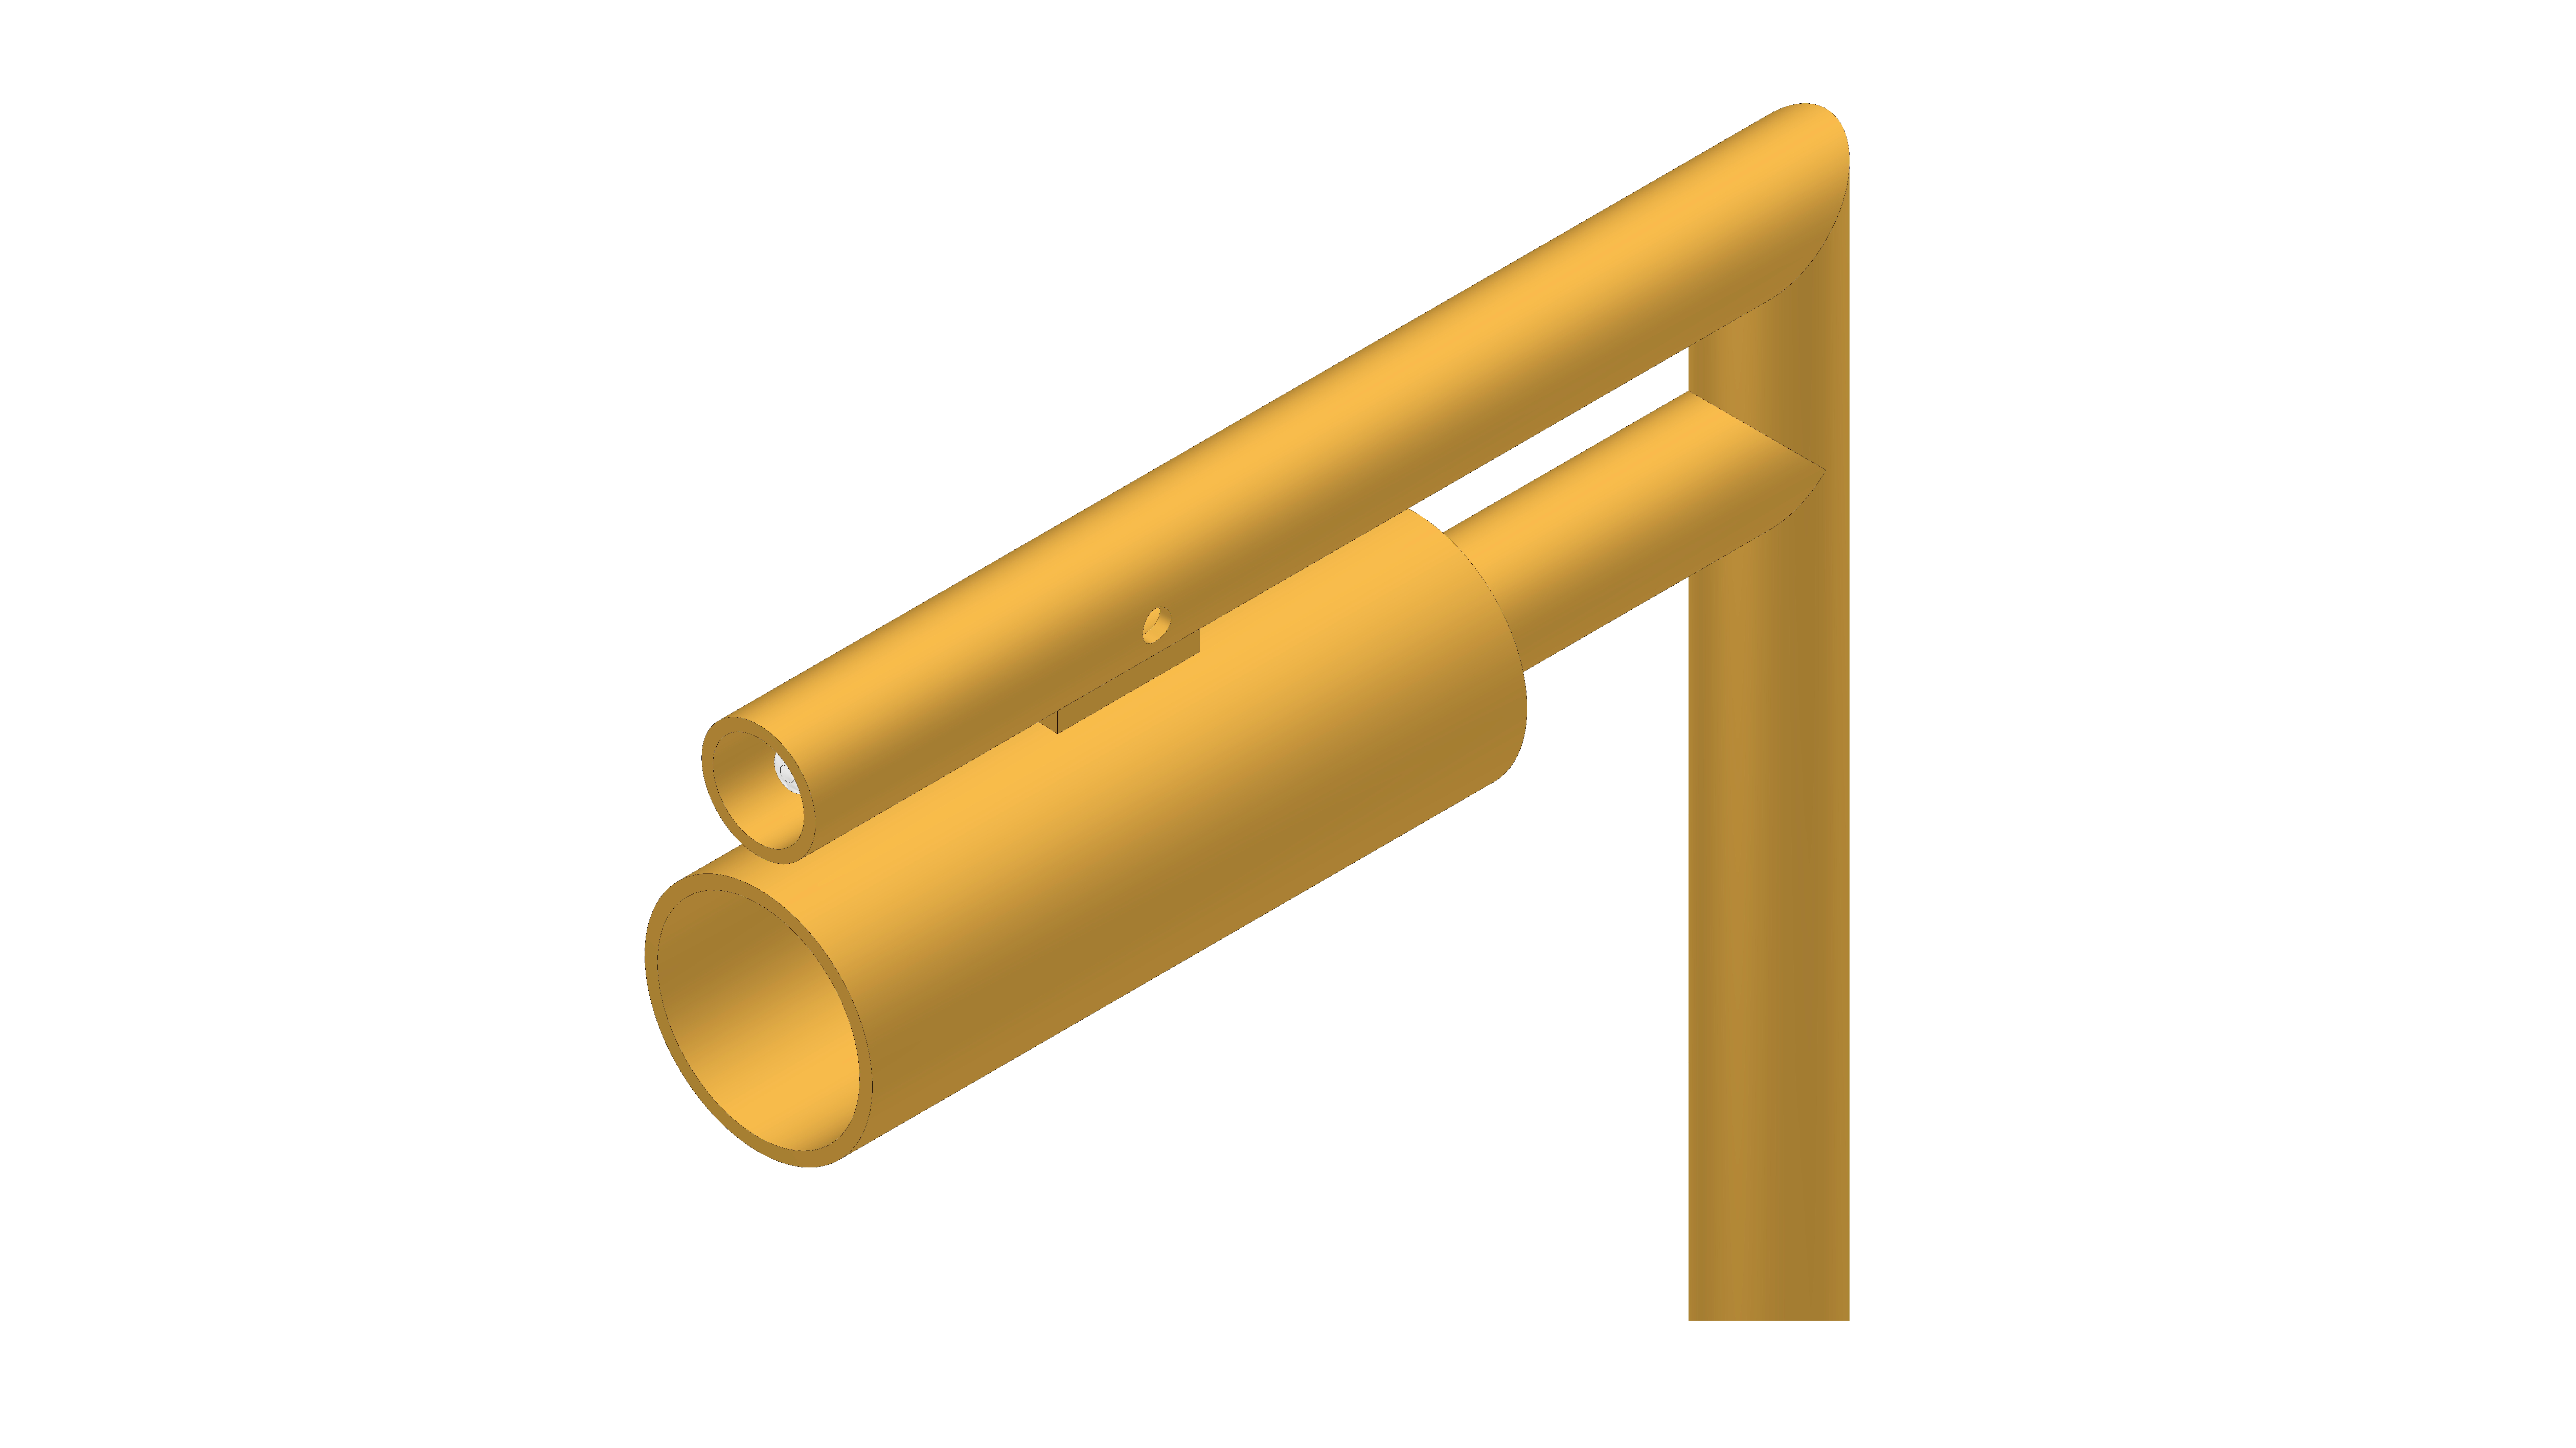
\includegraphics[width=\textwidth]{400_SIMULACE_KONSTRUKCNICH_UPRAV/Vykresy_rendery/Sonda_s_rozsirenym_stinenim_B.png}
            \caption{Sonda se stíněním čidla B}
            \label{fig:sonda-s-rozsirenym-stinenim-B}
        \end{figure}
        
        \subsubsection{Chování při různých rychlostech proudění}
            DATA
            
            \begin{figure}[ht!]
                \centering
                \includegraphics*[width=\textwidth, trim={5.9cm 1.0cm 5.8cm 2.0cm}]{400_SIMULACE_KONSTRUKCNICH_UPRAV/Grafy/03_rychlosti.eps}
                \caption{Závislost restitučních faktorů sondy s rozšířeným stíněním čidla B na rychlosti proudění}
                \label{fig:sonda-s-rosirenym-stinenim-rychlosti}
            \end{figure}
        \subsubsection{Směrová citlivost v rovině symetrie}
            DATA
            
            \begin{figure}[ht!]
                \centering
                \includegraphics*[width=\textwidth, trim={5.9cm 1.0cm 5.8cm 2.0cm}]{400_SIMULACE_KONSTRUKCNICH_UPRAV/Grafy/03_rovina_symetrie}
                \caption{Závislost restitučních faktorů sondy s rozšířeným stíněním čidla B na natočení sondy v rovině symetrie}
                \label{fig:sonda-s-rosirenym-stinenim-rovina-symetrie}
            \end{figure}
        \subsubsection{Směrová citlivost kolmo na rovinu symetrie}
            DATA
            
             \begin{figure}[ht!]
                \centering
                \includegraphics*[width=\textwidth, trim={5.9cm 1.0cm 5.8cm 2.0cm}]{400_SIMULACE_KONSTRUKCNICH_UPRAV/Grafy/03_kolma_rovina}
                \caption{Závislost restitučních faktorů sondy s rozšířeným stíněním čidla B na natočení kolmo na rovinu symetrie}
                \label{fig:sonda-s-rosirenym-stinenim-kolma-rovina}
            \end{figure}
        
    \newpage
    \subsection{Vliv průměru stínění čidla B}
        DATA
        
        \begin{figure}[ht!]
            \centering
            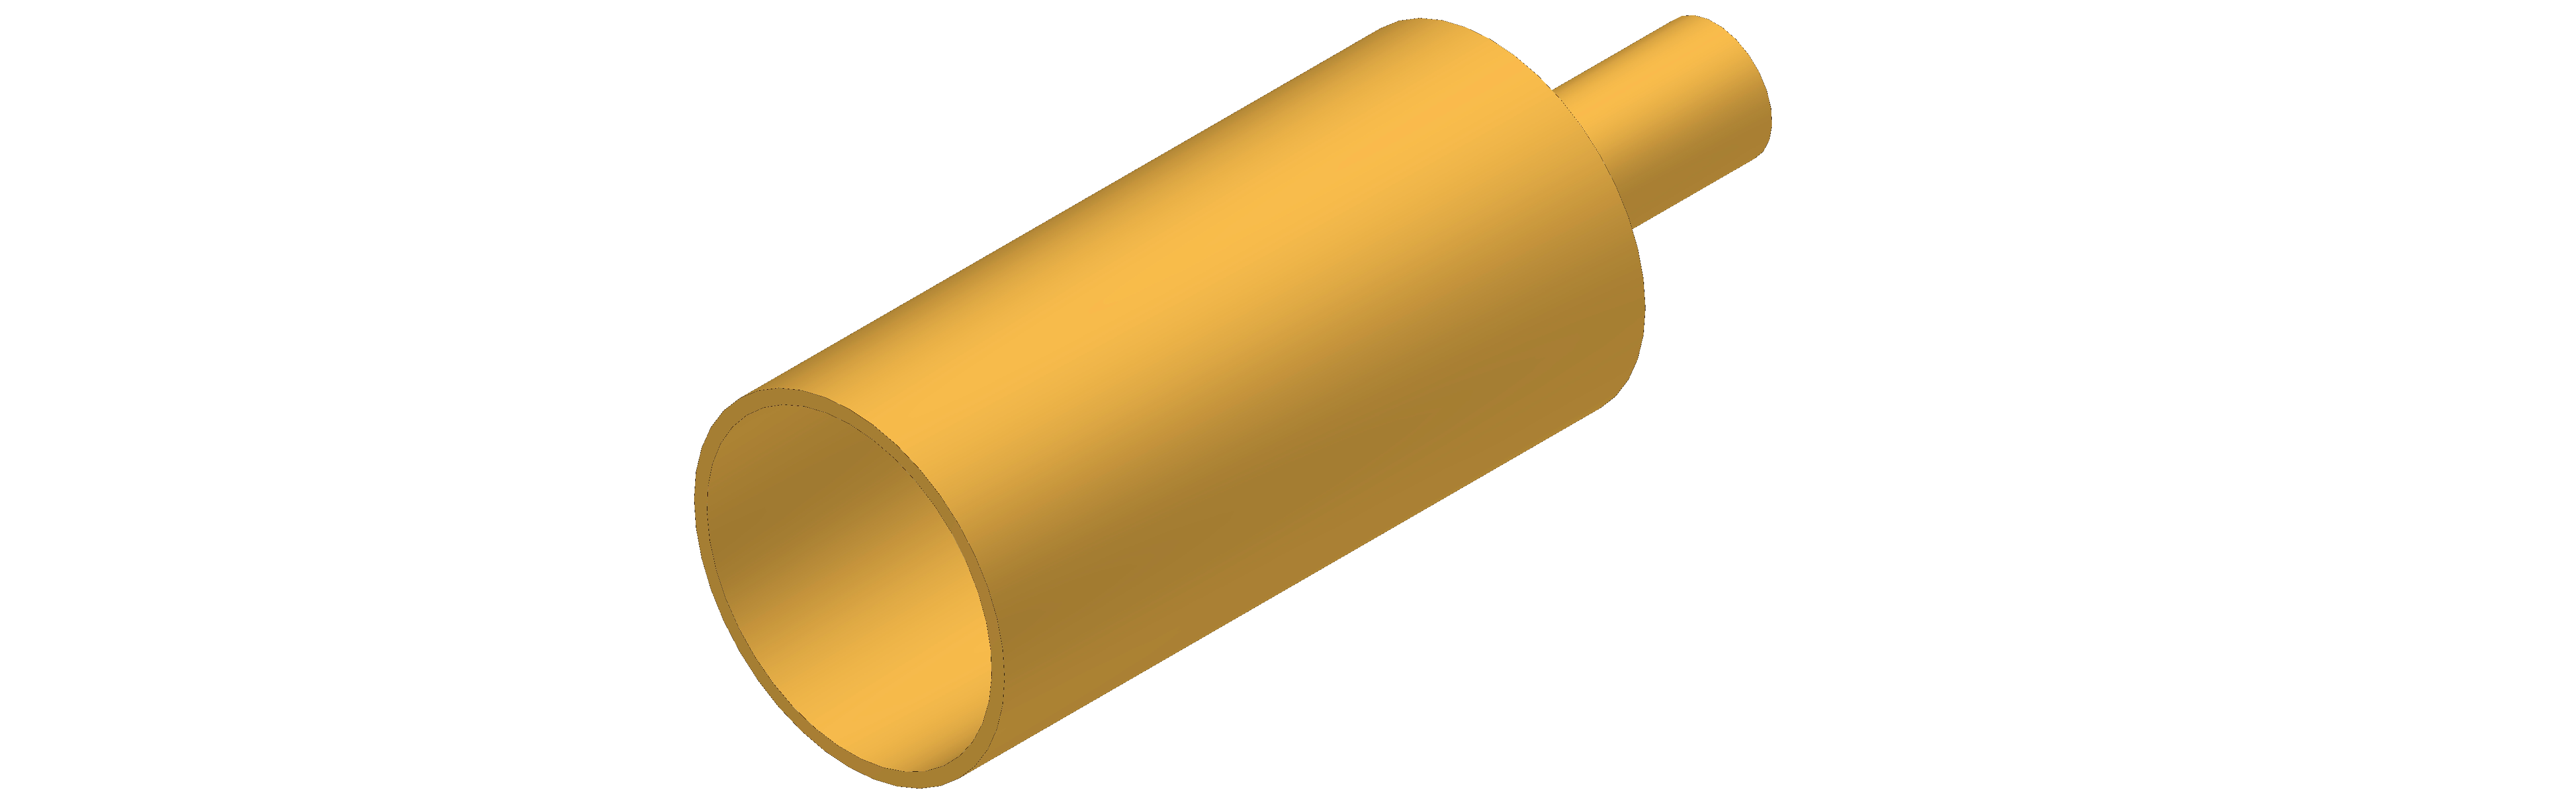
\includegraphics[width=\textwidth]{400_SIMULACE_KONSTRUKCNICH_UPRAV/Vykresy_rendery/Stineni_B.png}
            \caption{Stínění čidla B}
            \label{fig:stineni-B}
        \end{figure}
        
        
        \begin{figure}[ht!]
            \centering
            \includegraphics*[width=\textwidth, trim={5.9cm 1.0cm 5.8cm 2.0cm}]{400_SIMULACE_KONSTRUKCNICH_UPRAV/Grafy/04_prumer_stineni_B}
            \caption{Závislost restitučního faktoru čidla B na průměru stínění}
            \label{fig:prumer-stineni-B}
        \end{figure}
    
    \newpage
    \subsection{Vliv průměru stínění čidla A} \label{sec:stineni-A}
        DATA
        
        \begin{figure}[ht!]
            \centering
            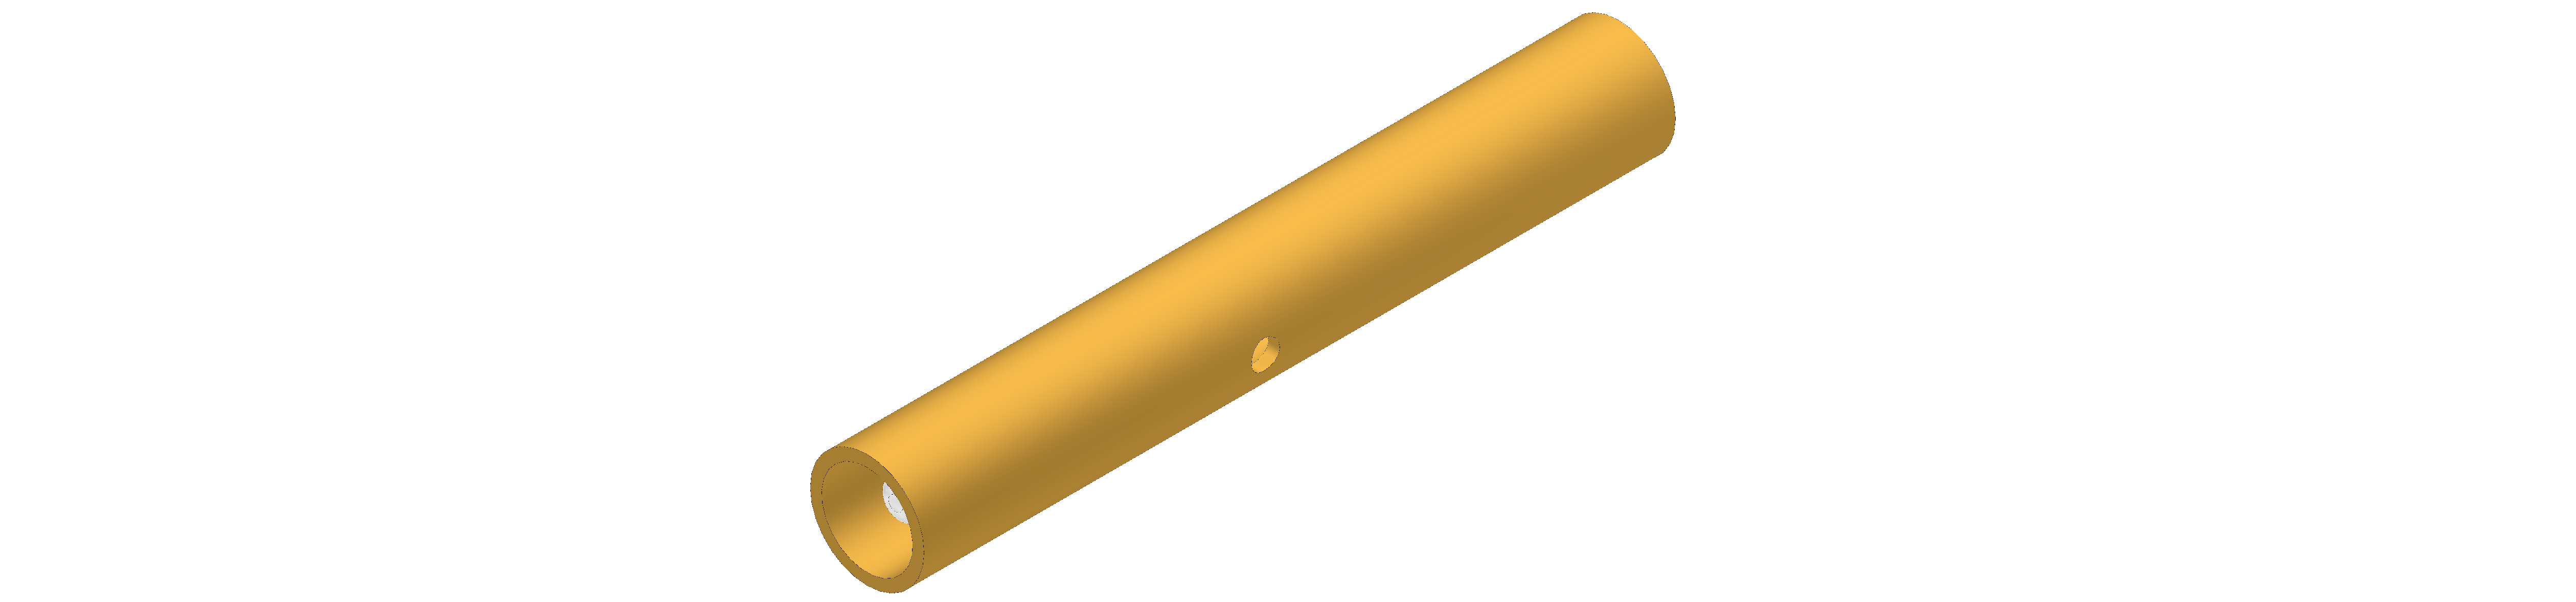
\includegraphics[width=\textwidth]{400_SIMULACE_KONSTRUKCNICH_UPRAV/Vykresy_rendery/Stineni_A.png}
            \caption{Stínění čidla A}
            \label{fig:stineni-A}
        \end{figure}
        
        \begin{figure}[ht!]
            \centering
            \includegraphics*[width=\textwidth, trim={5.25cm 1.0cm 5.8cm 2.0cm}]{400_SIMULACE_KONSTRUKCNICH_UPRAV/Grafy/05_prumer_stineni_A}
            \caption{Závislost restitučního faktoru čidla A na průměru stínění}
            \label{fig:prumer-stineni-A}
        \end{figure}
    
   \newpage
     \subsection{Vliv polohy odvětrání čidla A}
        DATA
        
          \begin{figure}[ht!]
            \centering
            \includegraphics*[width=\textwidth, trim={5.25cm 1.0cm 5.8cm 2.0cm}]{400_SIMULACE_KONSTRUKCNICH_UPRAV/Grafy/06_poloha_odvetrani_A.eps}
            \caption{Závislost restitučního faktoru čidla A na poloze odvětrání}
            \label{fig:poloha-odvetrani-A}
        \end{figure}
    
    \newpage
    \subsection{Vliv průměru odvětrání čidla A}
        DATA
        
        \begin{figure}[ht!]
            \centering
            \includegraphics*[width=\textwidth, trim={5.25cm 1.0cm 5.8cm 2.0cm}]{400_SIMULACE_KONSTRUKCNICH_UPRAV/Grafy/07_prumer_odvetrani_A.eps}
            \caption{Závislost restitučního faktoru čidla A na průměru odvětrání}
            \label{fig:prumer-odvetrani-A}
        \end{figure}
    
    \newpage
    \subsection{Vliv přidání divergentního vstupu pro čidlo A}
        DATA
        
        \begin{figure}[ht!]
            \centering
            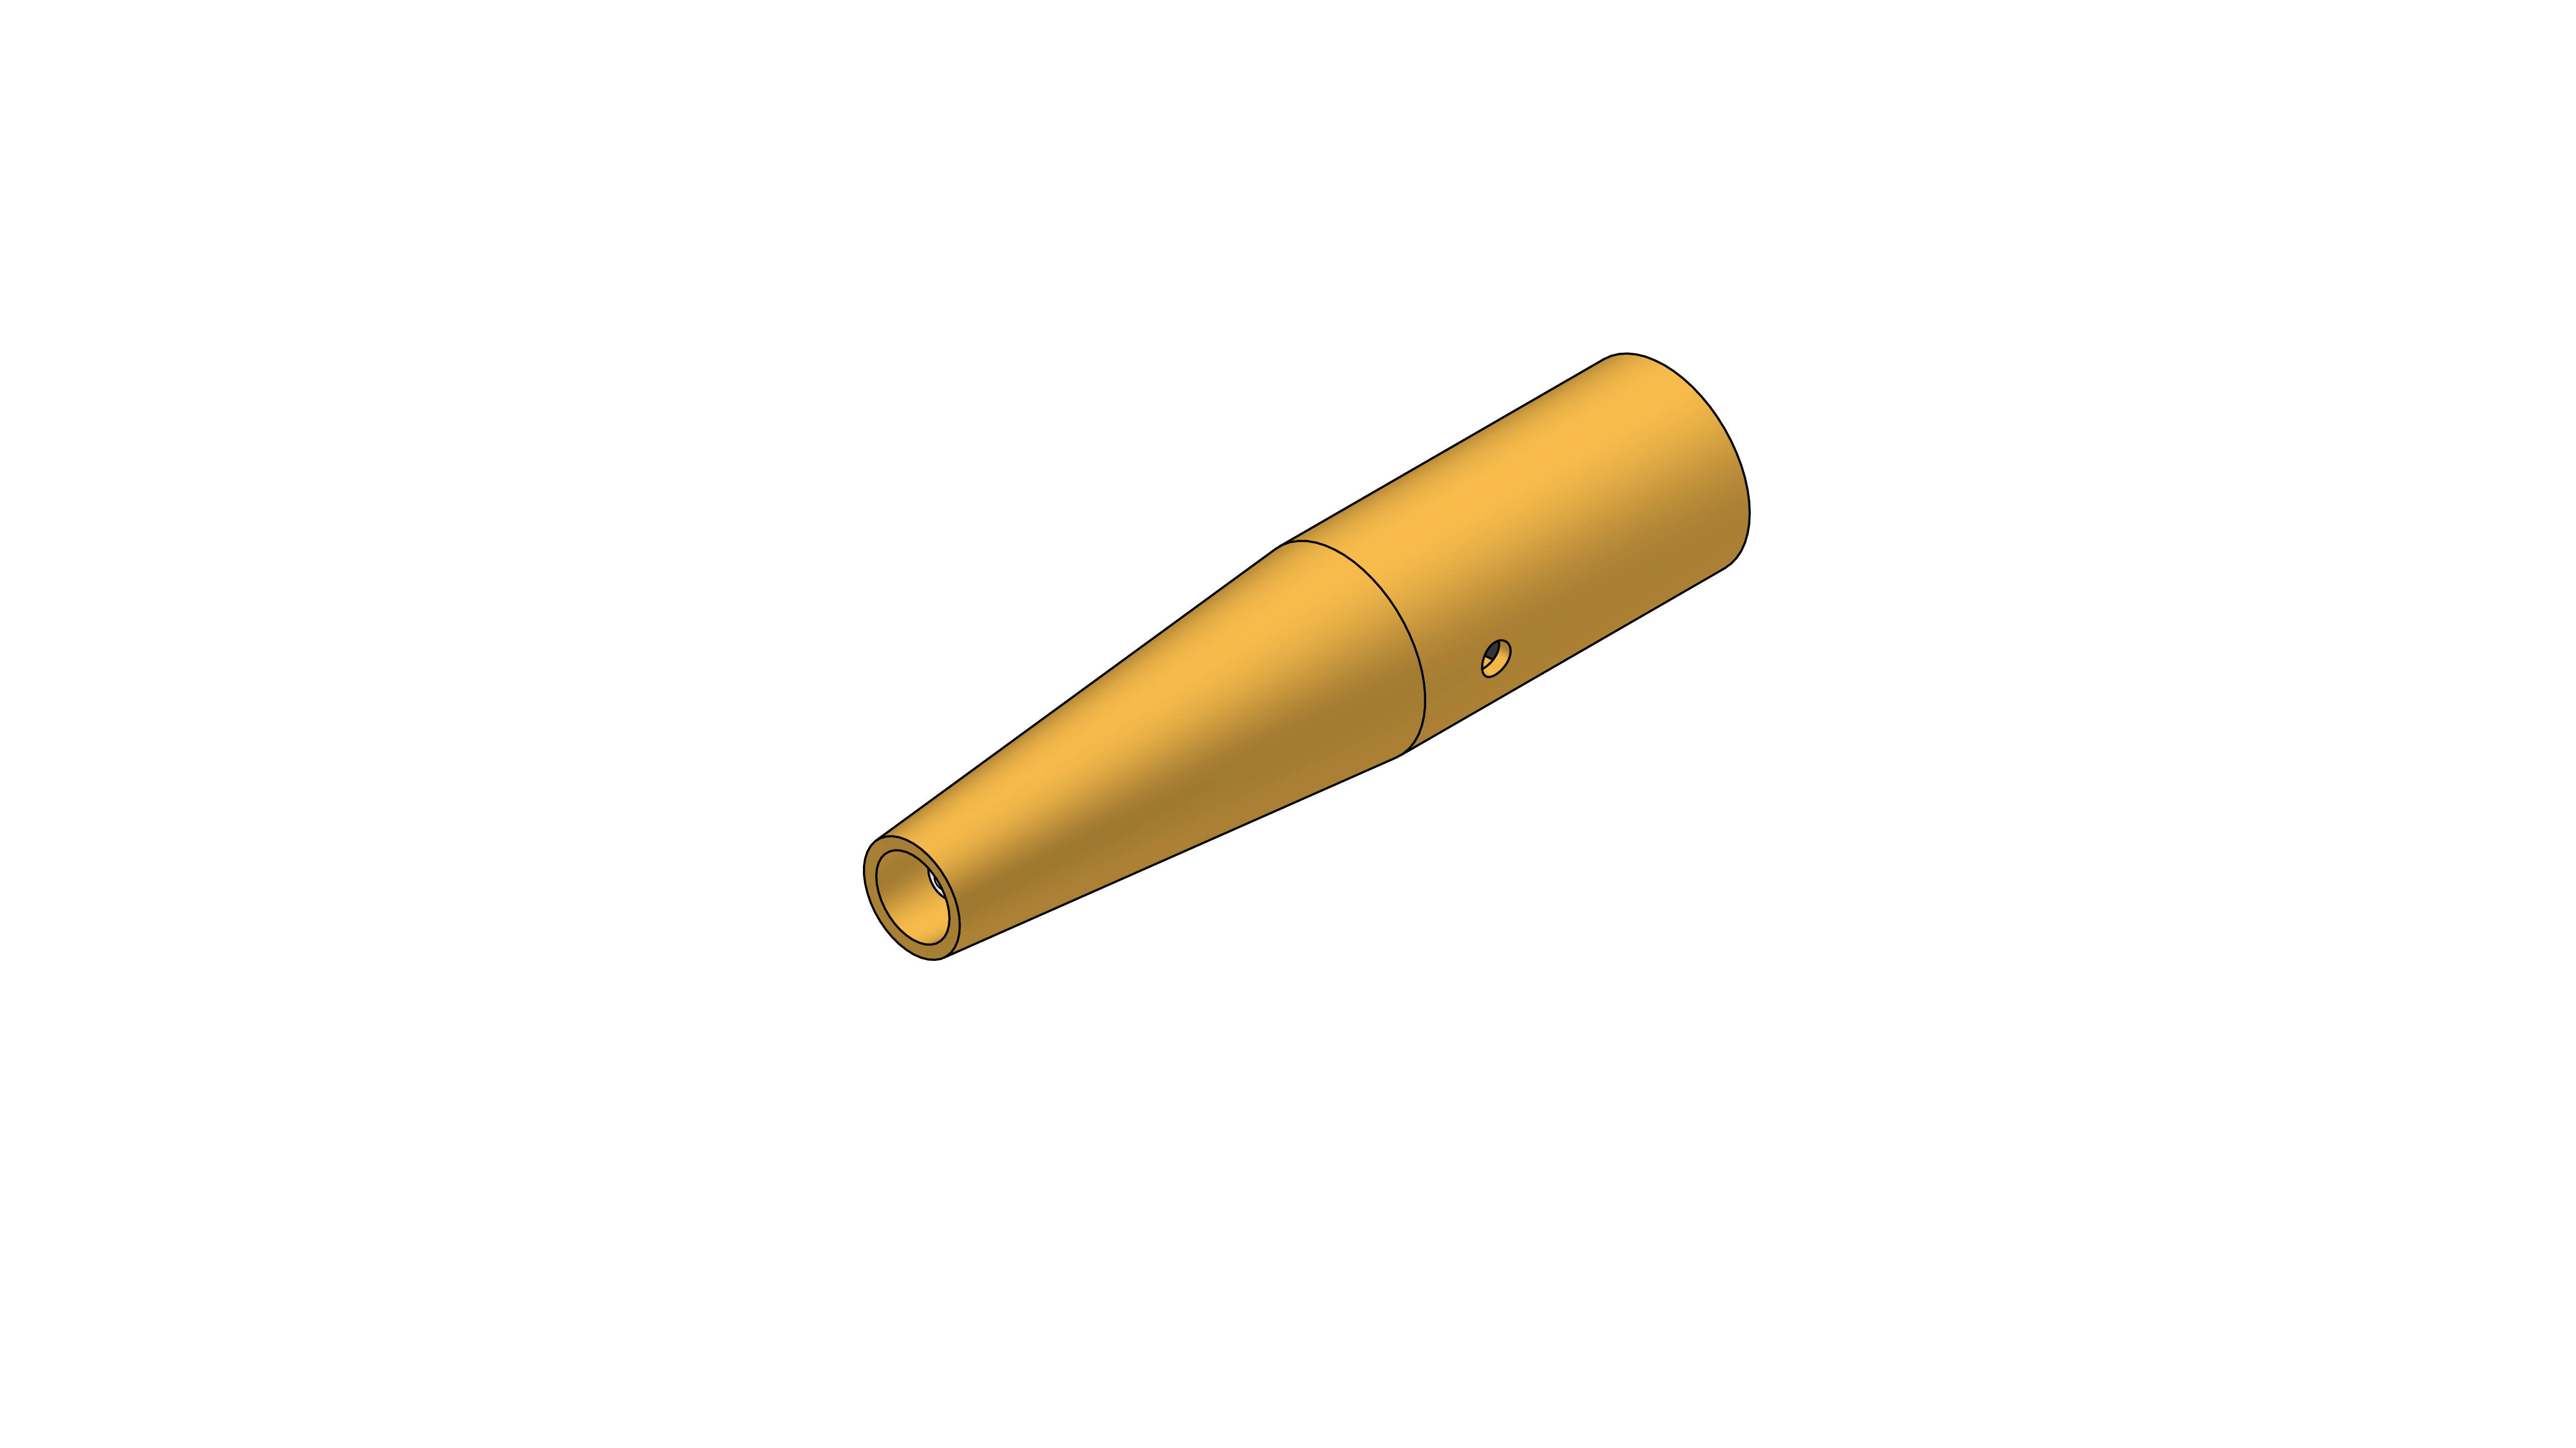
\includegraphics[width=\textwidth]{400_SIMULACE_KONSTRUKCNICH_UPRAV/Vykresy_rendery/Difuzor_A.png}
            \caption{Čidlo A s divergentním vstupem}
            \label{fig:difuzor-A}
        \end{figure}
    
        \begin{figure}[ht!]
            \centering
            \includegraphics*[width=\textwidth, trim={5.25cm 1.0cm 5.8cm 2.0cm}]{400_SIMULACE_KONSTRUKCNICH_UPRAV/Grafy/08_divergentni_cast_A.eps}
            \caption{Závislost restitučního faktoru čidla A na vrcholovém úhlu divergentního vstupu}
            \label{fig:divergentni-cast-A}
        \end{figure}
    
    \newpage
    \subsection{Vliv přidání kavity do stínění čidla A}
        DATA
        
        \begin{figure}[ht!]
            \centering
            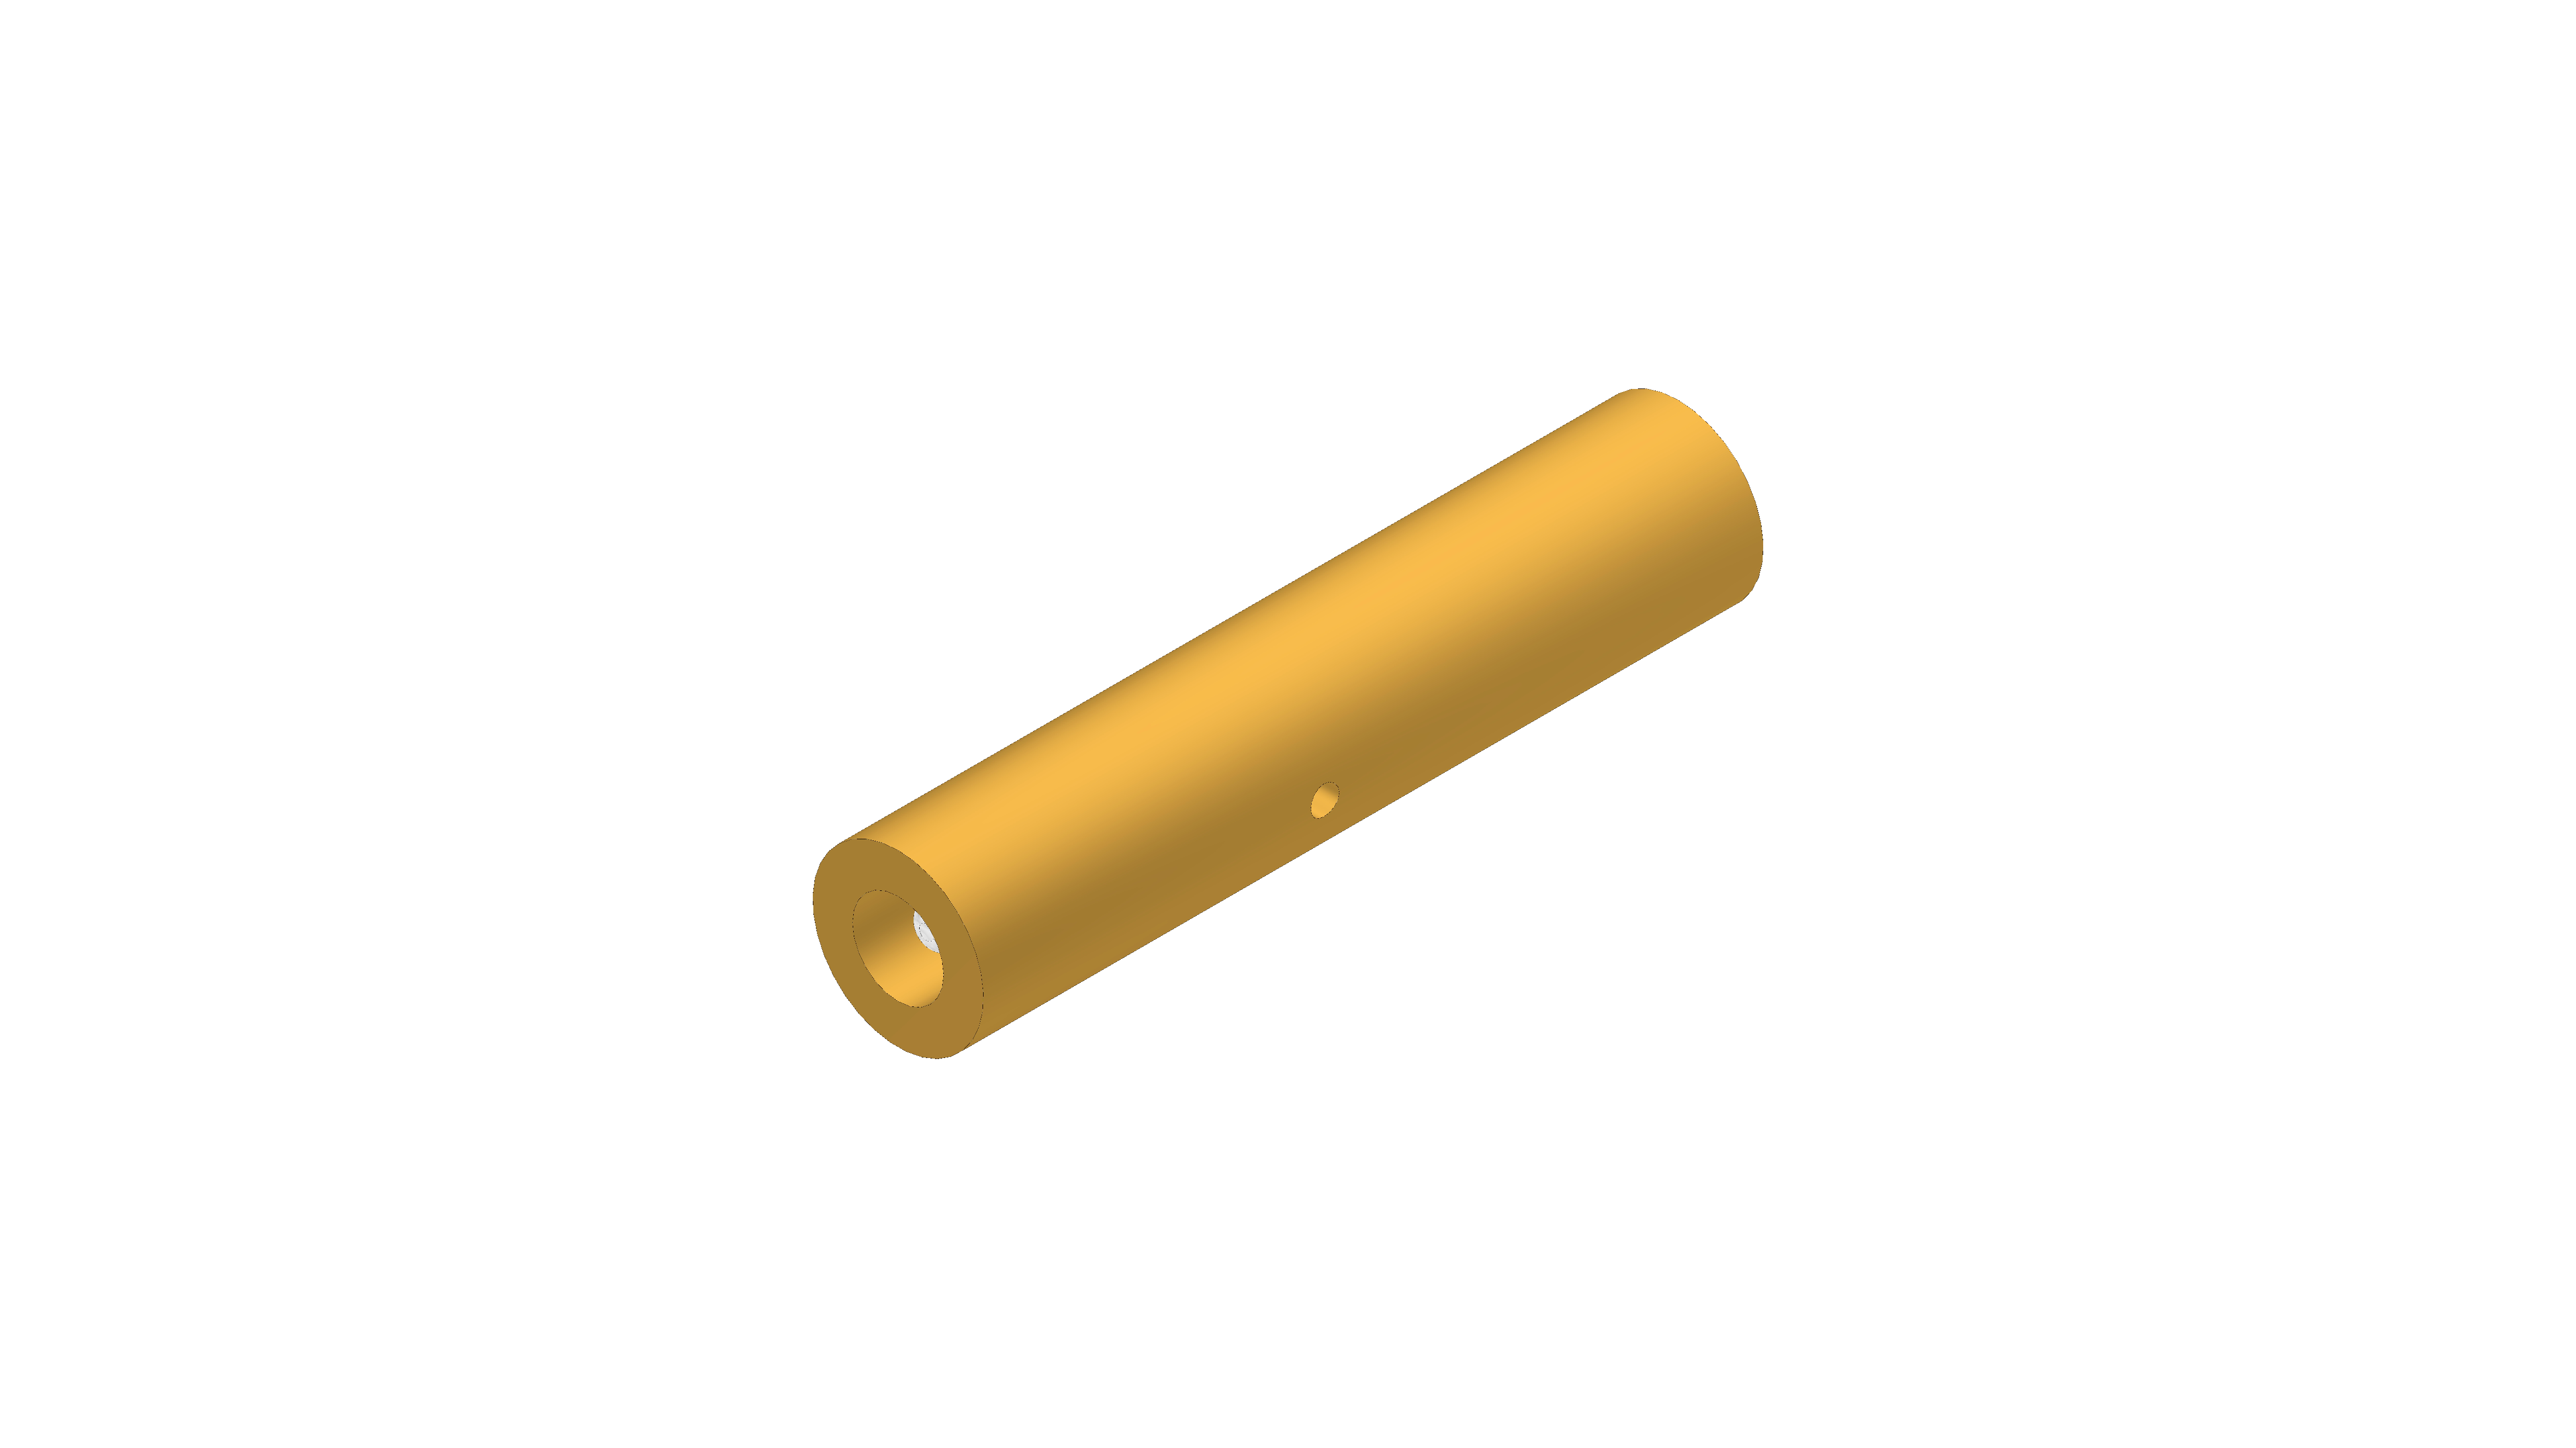
\includegraphics[width=\textwidth]{400_SIMULACE_KONSTRUKCNICH_UPRAV/Vykresy_rendery/Kavita.png}
            \caption{Čidlo A s přidanou kavitou do stínění}
            \label{fig:kavita-A}
        \end{figure}
    
        \begin{figure}[ht!]
            \centering
            \includegraphics*[width=\textwidth, trim={5.25cm 1.0cm 5.8cm 2.0cm}]{400_SIMULACE_KONSTRUKCNICH_UPRAV/Grafy/kavita.eps}
            \caption{Závislost restitučního faktoru čidla A na tloušťce kavity uvnitř stínění}
            \label{fig:kavita-A-graf}
        \end{figure}
    
    \newpage
    
    \subsection{Vliv přidání kavity do stínění čidla B}
        DATA
        
        \begin{figure}[ht!]
            \centering
            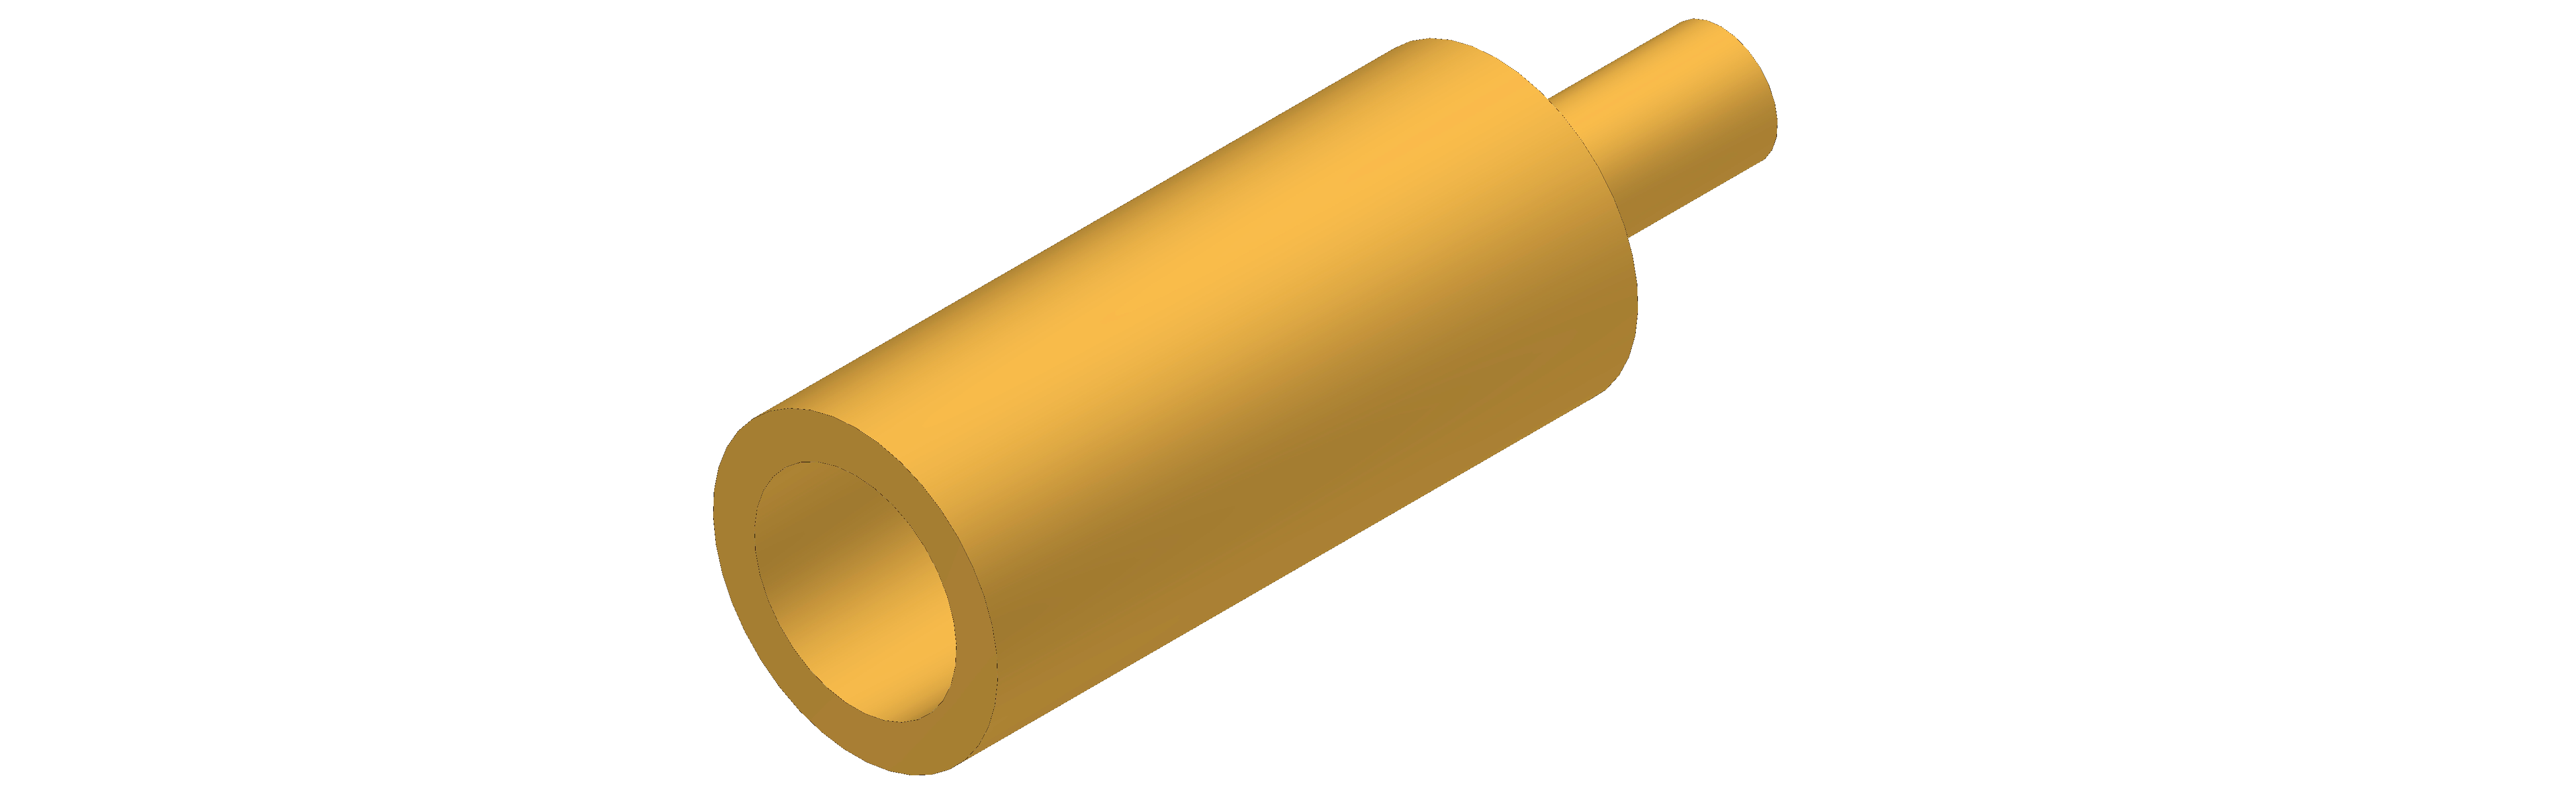
\includegraphics[width=\textwidth]{400_SIMULACE_KONSTRUKCNICH_UPRAV/Vykresy_rendery/Kavita_B.png}
            \caption{Čidlo B s přidanou kavitou do stínění}
            \label{fig:kavita-B}
        \end{figure}
    
        \begin{figure}[ht!]
            \centering
            \includegraphics*[width=\textwidth, trim={5.25cm 1.0cm 5.8cm 2.0cm}]{400_SIMULACE_KONSTRUKCNICH_UPRAV/Grafy/kavita_B.eps}
            \caption{Závislost restitučního faktoru čidla B na tloušťce kavity uvnitř stínění}
            \label{fig:kavita-B-graf}
        \end{figure}
    
    \newpage
    \subsection{Vliv materiálu trubice sondy}
        TODO
    